\documentclass{article} % \documentclass{} is the first command in any LaTeX code.  It is used to define what kind of document you are creating such as an article or a book, and begins the document preamble
\usepackage{pdfpages}
\usepackage{amsmath} % \usepackage is a command that allows you to add functionality to your LaTeX code
\usepackage{mathtools}
\usepackage{graphicx}

\DeclarePairedDelimiter{\opair}{\langle}{\rangle}

\title{Math 215 Homework 6 Problem 5} % Sets article title
\author{} % Sets authors name
\date{} % Sets date for date compiled

% The preamble ends with the command \begin{document}
\begin{document} % All begin commands must be paired with an end command somewhere
    \maketitle
    Sketch a graph of the function $f$(x,y) = $\sqrt{4x^2+y^2}$\\\\
    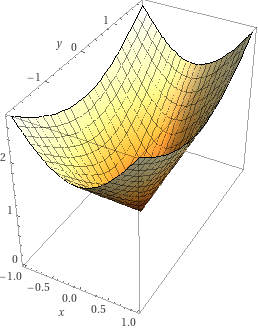
\includegraphics{image.png}



\end{document}